%
%  Antrag, Aufgabenstellung Diplomarbet
%
%  Created by Silvan Spross on 2011-02-03.
%
\documentclass[]{scrreprt}
\usepackage[ngerman]{babel}

% Use utf-8 encoding for foreign characters
\usepackage[utf8]{inputenc}

% Setup for fullpage use
\usepackage{fullpage}

% Package for including code in the document
\usepackage{listings}

% If you want to generate a toc for each chapter (use with book)
\usepackage{minitoc}

% This is now the recommended way for checking for PDFLaTeX:
\usepackage{ifpdf}

\usepackage{ulem}

\ifpdf
    \usepackage[pdftex]{graphicx}
\else
    \usepackage{graphicx}
\fi

\title{Evaluation Vorgehensmodell}
    
\author{Silvan Spross}
    
\date{13. April 2011}

\begin{document}

    \ifpdf
        \DeclareGraphicsExtensions{.pdf, .jpg, .tif}
    \else
        \DeclareGraphicsExtensions{.eps, .jpg}
    \fi

    \maketitle

    \pagenumbering{arabic}

    % \tableofcontents

    \chapter{Vorgehensmodelle}

    \section{Workflow Management}
    Das Workflow-Management umfasst alle Aufgaben, die bei der Modellierung, 
    Spezifikation, Simulation sowie bei der Ausführung und Steuerung der 
    Workflows erfüllt werden müssen.
    
    Eine Aktivität bildet die kleinste Ausführungseinheit in einem Arbeitsablauf. 
    Dieser Aktivität sind typischerweise eine Tätigkeit, ausführende Ressourcen 
    (Personen, Maschinen), zu benutzende Ressourcen (Werkzeuge, Maschinen, andersweitige Betriebsmittel) 
    und zeitliche Abhängigkeit (Reihenfolge, Ausführungsdauer usw.) zugeordnet.
    
    \begin{itemize}
        \item Durch den Workflowplan lassen sich Fehler einem einzelnen Team und oder einem bestimmten Mitarbeiter zuordnen. Daraus folgt die Tendenz bei den Beteiligten, eher untätig zu bleiben, als einen Fehler zu machen, sich möglichst gut abzusichern und den schwarzen Peter anderen zuzuschieben.
        \item Das Management betrachtet Mitarbeiter potentiell als austauschbare Ressourcen zur Erfüllung des Workflowplans. Das kann die wichtige Beziehung zwischen Führung und Mitarbeiterkörper empfindlich stören.
        \item Kreativität und Ideen zur Verbesserung der Geschäftsprozesse werden durch den gegebenen Rahmen eher gebremst.
    \end{itemize}
    
    \section{Change Management nach Lewin}
    \subsection{Auftauphase (unfreezing)}
    Ausgangspunkt der ersten Phase ist die Einsicht, dass die Erwartungen nicht mehr der Realität entsprechen. Die Notwendigkeit einer Veränderung tritt langsam als Möglichkeit ins Bewusstsein und altes Verhalten wird in Frage gestellt. Addiert man nun die gewisse und nötige Flexibilität, kann die Bereitschaft für Veränderungen entstehen. Das generelle Ziel dieser Phase besteht darin, die nach Veränderung strebenden Kräfte zu stärken und zu unterstützen und so ein Veränderungsbewusstsein zu induzieren. Unfreezing steht dabei bildlich für das Auftauen des bestehenden (eingefrorenen) Gleichgewichtes oder des zuvor erreichten Zustands, der auch wiederum aus einem vorangegangenen Change-Prozess hervorgerufen worden sein kann.
    
    \subsection{Bewegungsphase (moving)}
    In der zweiten Phase, der Moving- oder Veränderungsphase, werden Lösungen generiert, neue Verhaltensweisen ausprobiert und das Problem wird in Teilprojekten gelöst. Der Status-quo wird verlassen und es wird eine verändernde Bewegung zu einem neuen Gleichgewicht vollzogen.
   
    \subsection{Einfrierphase (refreezing)}
    Ziel der dritten Phase, dem Wieder-Einfrieren, ist die Implementierung der gefundenen Problemlösungen und damit der zumindest vorläufige Abschluss des Veränderungsprozesses. Nach dem Episodenschema von Lewin bedürfen durchgeführte Veränderungen der Stabilisierung und müssen zur dauerhaften Integration in das Gesamtsystem wieder eingefroren werden. Der neue Gleichgewichtszustand soll so vor der Macht der Gewohnheit geschützt und stabilisiert werden. Fazit: Aus „neu“ mach „alt“ im positiven Sinne des Bekannten, Vertrauten und Funktionierenden.
    
    \subsection{Acht Schritte zum Veränderungserfolg empfiehlt Kotter}
    \begin{enumerate}
        \item Bewusstsein für die Dringlichkeit schaffen
        \item Verantwortliche mit Veränderungsbereitschaft gewinnen und zusammenbringen
        \item Die Zukunftsvision ausformulieren und eine Strategie entwickeln, wie Sie dahin kommen
        \item Die Zukunftsvision bekannt machen
        \item Handeln im Sinne der neuen Vision und der Ziele ermöglichen
        \item Kurzfristige Erfolge planen und gezielt herbeiführen
        \item Erreichte Verbesserungen systematisch weiter ausbauen
        \item Das Neue fest verankern
    \end{enumerate}
    
    \section{St. Galler Management-Modell}
    \begin{figure}[htbp]
    \begin{center}
    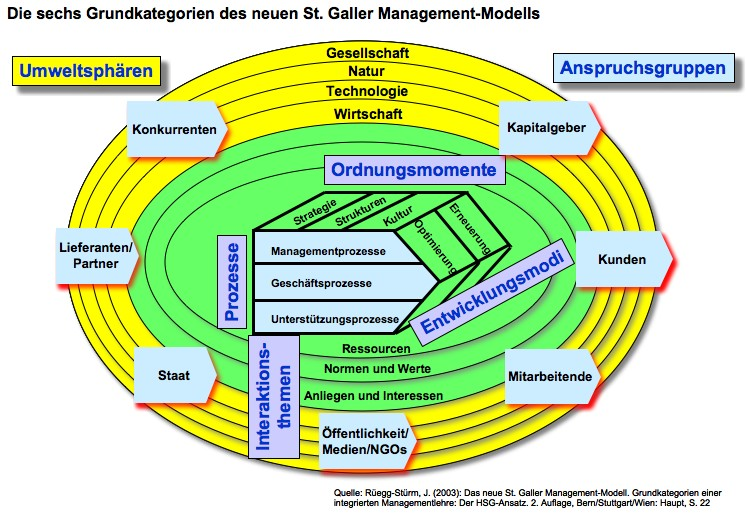
\includegraphics[width=0.7\textwidth,angle=0]{./st_galler.jpg}
    \caption{St. Galler Manamgement-Modell}
    \label{pic:st_galler}
    \end{center}
    \end{figure}
    
    \clearpage
    
    \section{Balanced Scorecards}
    \subsection{Perspektiven der BSC}
    \begin{itemize}
        \item Finanzperspektive: Kennzahlen zum Erreichen der finanziellen Ziele.
        \item Kundenperspektive: Kennzahlen zum Erreichen der Kundenziele.
        \item Interne bzw. Prozessperspektive: Kennzahlen zum Erreichen der internen Prozess- und Produktionsziele.
        \item Mitarbeiter-, Potenzial- bzw. Lern- und Wachstumsperspektive: Kennzahlen zum Erreichen der (langfristigen) Überlebensziele der Organisation.
    \end{itemize}
    Grundsätzlich gut, benötigt aber sehr viel Zeit für Datenerfassung und Analyse.
    
    \section{HERMES}
    HERMES ist eine offene Methode, um Projekte der Informations- und Kommunikationstechnik (IKT) einheitlich und strukturiert durchzuführen. Die Methode ist in der Bundesverwaltung verbindlich und muss bei allen  IKT-Projekten angewendet werden. HERMES wird auch in anderen öffentlichen Verwaltungen sowie Lehrinstituten und Unternehmen eingesetzt.
    
    Zu IT lastig.
    
    \section{ITIL}
    Ebenfalls zu IT lastig.
    
    \begin{figure}[htbp]
    \begin{center}
    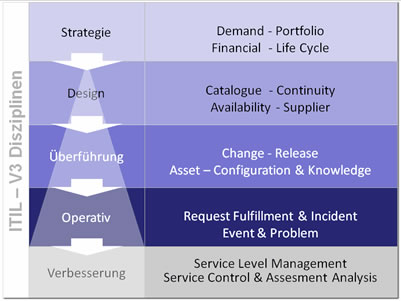
\includegraphics[width=0.6\textwidth,angle=0]{./itil.jpg}
    \caption{ITIL Disziplinen}
    \label{pic:itil}
    \end{center}
    \end{figure}
    
    \clearpage
    
    \section{RUP}
    Der Rational Unified Process (RUP) ist ein kommerzielles Produkt der Firma Rational Software, die seit 2003 Teil des IBM-Konzerns ist. Es beinhaltet sowohl ein Vorgehensmodell zur Softwareentwicklung als auch die dazugehörigen Softwareentwicklungsprogramme.
    
    Zu IT lastig.
    
    \section{Vorgehensmodell nach Grochla}
    \subsection{Voruntersuchung}
    In der Voruntersuchung, auch Pilotstudie genannt, stellt man sich Fragen wie
    ``Was soll geändert werden?'' und ``Welches sind die Ziele?''. Man verschafft
    sich einen Grobüberblick über das eigentliche Problem und die Rahmenbedingungen
    möglicher Lösungen. Auch entscheidet man in der Voruntersuchung, ob der Prozess
    fortgesetzt oder abgebrochen werden soll. In der Voruntersuchung können die 
    meisten Analyse- und Bewertungstechniken verwendet werden.

    \subsection{Ist-Aufnahme}
    In der zweiten Phase erfasst man den aktuellen Zustand indem man das zu 
    Untersuchende aus möglichst vielen Betrachtungswinkeln analysieren. Zu den
    Techniken der Ist-Aufnahme zählen die Selbstaufschreibung, die Befragung und 
    die Beobachtung.

    \subsection{Ist-Kritik}
    In der dritten Phase widmet man sich den erhobenen Informationen aus der zweiten Phase. 
    Die genauen Ursachen der Probleme sollen herausgeschält werden, damit nicht nur 
    Symptome behandelt werden.
    
\end{document}